% ==============================================================================
\section{Módulo de Ray Casting}
\label{sec:dev_ray}
% ==============================================================================

\subsection{Descripción}

El módulo de Ray Casting, implementado en \texttt{occupancy\_grid.py}, es el puente
entre las observaciones del SLAM y el mapa de ocupación. En el sistema final cumple
dos funciones distintas que comparten el mismo núcleo de recorrido de celdas:

\begin{enumerate}
    \item \textbf{Actualización del mapa.} Desde la pose estimada se traza un rayo por
    cada observación; las celdas atravesadas acumulan evidencia de espacio libre y la
    celda del extremo acumula evidencia de ocupación. Esto corresponde al modelo
    inverso del sensor de los mapas de ocupación \cite{moravec1985sonar, elfes1989}.
    \item \textbf{Consulta del mapa.} Desde la pose actual se lanzan rayos virtuales
    sobre el mapa ya construido para medir la distancia libre en cada dirección. Estas
    distancias son las variables $d_{\text{front}}$, $d_{\text{left}}$ y
    $d_{\text{right}}$ que recibe el módulo de navegación.
\end{enumerate}

En el diseño de TT1 solo se contemplaba la primera función con la regla básica ``libre
en el recorrido, ocupado al final''. Durante el desarrollo esa regla resultó
insuficiente porque las observaciones del sistema tienen precisiones muy distintas
(5~cm del ultrasonido frente a $\pm 30$\,\% de la estimación monocular), por lo que se
añadieron las reglas descritas en esta sección.

\subsection{Discretización y recorrido de celdas}

El plano se discretiza en celdas de $5 \times 5$~cm. Un punto $(x, y)$ del mundo
corresponde a la celda $(\lfloor x / 0.05 \rfloor,\; \lfloor y / 0.05 \rfloor)$, y el
extremo de un rayo con rango $r$ y dirección relativa $\phi$ desde la pose
$(x, y, \theta)$ es:

\[
x_e = x + r\cos(\theta + \phi),
\qquad
y_e = y + r\sin(\theta + \phi)
\]

Las celdas atravesadas entre la celda del usuario y la del extremo se obtienen con el
algoritmo de Bresenham \cite{bresenham1965}, que avanza celda por celda utilizando
únicamente sumas y comparaciones de enteros (Figura~\ref{fig:ray_bresenham}). Para un
alcance máximo de 4~m, un rayo recorre a lo sumo 80 celdas. Se consideró el algoritmo
de recorrido de vóxeles de Amanatides y Woo \cite{amanatides1987voxel}, que visita
todas las celdas que toca el segmento, pero Bresenham resultó suficiente para la
actualización y es más sencillo; la consecuencia de esta elección en la consulta se
discute en las limitaciones.

\begin{figure}[H]
    \centering
    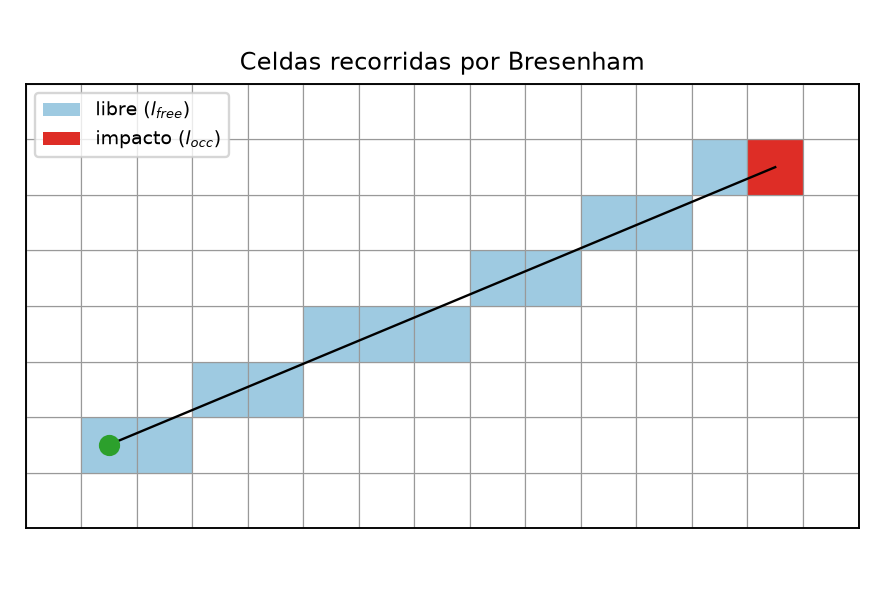
\includegraphics[width=0.6\textwidth]{Capturas_TT2/raycasting_bresenham.png}
    \caption{Celdas recorridas por el algoritmo de Bresenham para un rayo: las celdas
    intermedias reciben evidencia de espacio libre y la celda del extremo, de
    ocupación.}
    \label{fig:ray_bresenham}
\end{figure}

\subsection{Modelo inverso del sensor en log-odds}

Cada celda almacena el logaritmo de la razón de probabilidades de estar ocupada,
$l = \log\frac{p}{1-p}$, de modo que la fusión de una nueva observación es una suma
\cite{thrun2005probabilistic}. La probabilidad se recupera como
$p = 1/(1 + e^{-l})$. La Tabla~\ref{tab:ray_constantes} resume las constantes
utilizadas.

\begin{table}[H]
\centering
\caption{Constantes del modelo inverso del sensor}
\label{tab:ray_constantes}
\renewcommand{\arraystretch}{1.25}
\begin{tabular}{|p{2.6cm}|c|c|p{6.8cm}|}
\hline
\textbf{Constante} & \textbf{Log-odds} & \textbf{Probabilidad} & \textbf{Significado} \\
\hline
$l_{occ}$ & $+1.2$ & 0.77 & Incremento en la celda donde termina un rayo preciso. \\
\hline
$l_{free}$ & $-0.4$ & 0.40 & Incremento en cada celda atravesada. \\
\hline
$l_{\min}, l_{\max}$ & $\pm 5.0$ & 0.007 / 0.993 & Saturación de la celda. \\
\hline
Umbral de ocupado & $1.0$ & 0.73 & Por encima, la celda se considera obstáculo. \\
\hline
$L_{block}$ & $2.0$ & 0.88 & Por encima, la celda se considera una superficie
consolidada que detiene los rayos de espacio libre. \\
\hline
\end{tabular}
\end{table}

La asimetría entre $l_{occ}$ y $l_{free}$ es intencional: un rayo atraviesa muchas
celdas pero termina en una sola, por lo que la evidencia de ocupación debe pesar más
para que los obstáculos no se borren por los rayos que pasan junto a ellos. La
saturación en $\pm 5$ evita que una celda acumule tanta evidencia que después no pueda
corregirse \cite{hornung2013octomap}. La Figura~\ref{fig:ray_logodds} muestra el
efecto con las mismas reglas del código: una celda que se vio libre muchas veces
necesita seis impactos para volver a considerarse ocupada cuando aparece un
obstáculo. La figura también muestra la limitación discutida al final de esta
sección: una vez que la celda supera $L_{block}$, los rayos de espacio libre se
detienen en ella y su valor ya no disminuye aunque el obstáculo se retire.

\begin{figure}[H]
    \centering
    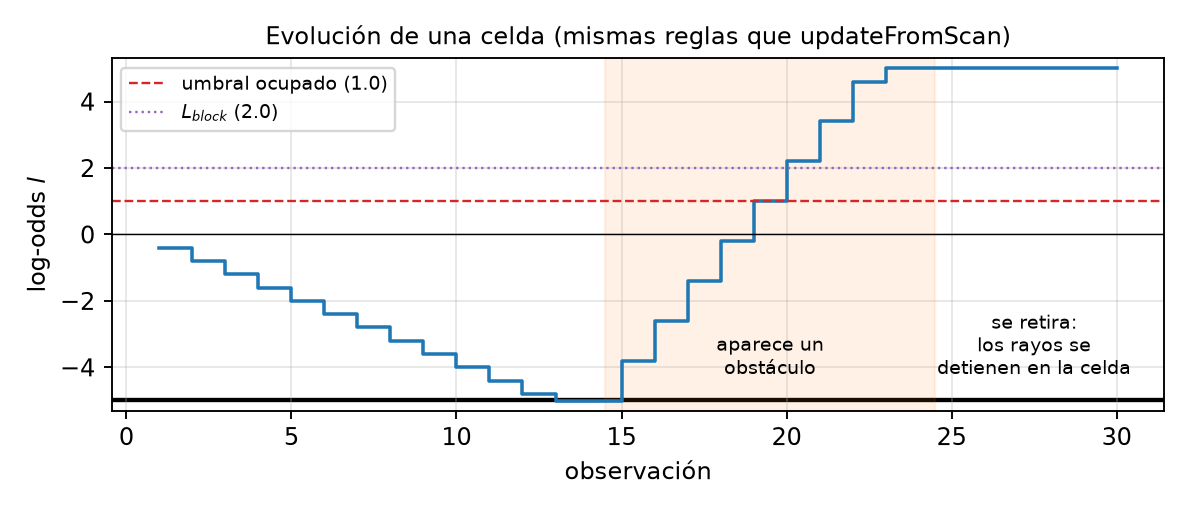
\includegraphics[width=0.82\textwidth]{Capturas_TT2/raycasting_logodds.png}
    \caption{Evolución del log-odds de una celda que primero se observa libre, después
    ocupada y finalmente queda libre otra vez, calculada con las reglas de
    \texttt{updateFromScan}.}
    \label{fig:ray_logodds}
\end{figure}

\subsection{Reglas añadidas durante el desarrollo}

Sobre el modelo básico se implementaron las siguientes reglas, cada una motivada por
un problema observado durante las pruebas:

\begin{enumerate}
    \item \textbf{El rango impreciso no marca ocupación.} Si la observación tiene
    $\sigma_r > 0.15$~m (estimación monocular cruda), el rayo solo despeja espacio
    libre hasta $r - 2\sigma_r$ y no marca la celda final como ocupada. El propósito
    es evitar que el ruido monocular deje manchas de celdas ocupadas alrededor de cada
    objeto y que despeje como libre el espacio donde realmente está el objeto. La
    ocupación de los objetos detectados por visión llega al mapa por la vía precisa:
    el rayo anclado a la posición consolidada del \emph{landmark} que genera el SLAM.
    \item \textbf{Las superficies consolidadas detienen el rayo.} Si al recorrer el
    rayo se encuentra una celda con $l > L_{block}$, el recorrido se detiene y no se
    marca nada más allá. Así un rayo ruidoso no perfora una pared ya registrada ni
    pinta marcas fantasma detrás de ella.
    \item \textbf{Rayos sin eco.} Cuando un sensor ultrasónico no recibe eco, se genera
    un rayo de espacio libre con la longitud del alcance máximo; como su extremo cae
    fuera del alcance útil, no marca ocupación. Esto permite registrar pasillos libres.
    \item \textbf{Recorte en lugar de descarte.} En la retícula de tamaño fijo, si el
    extremo de un rayo cae fuera del mapa, el rayo se recorta en el borde y se
    conservan las celdas libres recorridas. Inicialmente esos rayos se descartaban
    completos. En el mapa por bloques (Sección~\ref{sec:dev_mapeo}) esta regla deja de
    ser necesaria porque el mapa no tiene bordes.
    \item \textbf{Alcance máximo.} Los rayos se limitan a 4~m; una observación más
    lejana solo despeja espacio libre hasta ese límite.
    \item \textbf{Peligros de piso.} Las observaciones marcadas como peligro (hoyos,
    agua, escaleras) no modifican el log-odds, ya que el espacio por encima de un hoyo
    está libre; en su lugar suman un impacto en una capa separada que se describe en
    el módulo de mapeo.
\end{enumerate}

La Figura~\ref{fig:ray_casos} muestra el resultado de ejecutar el código del módulo en
tres casos representativos, con celdas de 10~cm para facilitar su lectura.

\begin{figure}[H]
    \centering
    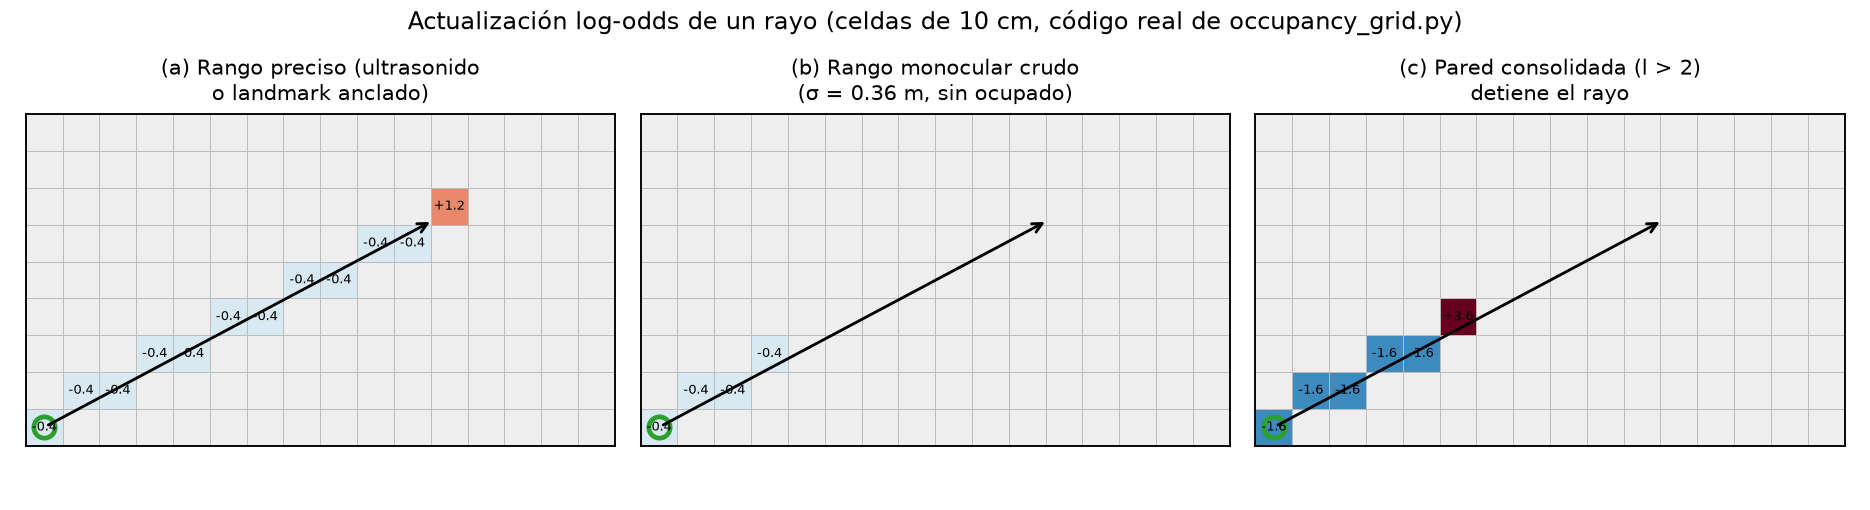
\includegraphics[width=\textwidth]{Capturas_TT2/raycasting_casos.png}
    \caption{Actualización de un rayo en tres casos: (a) rango preciso, que despeja el
    recorrido y marca el extremo; (b) rango monocular crudo, que solo despeja hasta
    $r - 2\sigma_r$; (c) rayo detenido por una superficie consolidada.}
    \label{fig:ray_casos}
\end{figure}

El Algoritmo~\ref{alg:dev_ray_update} describe la actualización tal como quedó
implementada en \texttt{updateFromScan}.

\begin{center}
\captionof{algorithm}{Actualización del mapa por Ray Casting}
\label{alg:dev_ray_update}
\end{center}
\vspace{-1.8cm}
\rule{\textwidth}{0.4pt}
\vspace{-0.9cm}
\begin{algorithmic}[1]

\Statex \textbf{ENTRADA:}
\Statex pose \Comment{(x, y, $\theta$) estimada por el SLAM}
\Statex observaciones \Comment{ancladas a landmarks + ecos + rayos sin eco}
\Statex alcance\_max \Comment{4 m}
\Statex \textbf{SALIDA:}
\Statex mapa actualizado (log-odds y capa de peligros)

\Statex
\State celda\_origen $\gets$ a\_celda(x, y)
\For{cada obs en observaciones}
    \State r $\gets$ mín(obs.r, alcance\_max)
    \State impreciso $\gets$ obs.$\sigma_r > 0.15$
    \State extremo $\gets$ a\_celda(x + r cos($\theta$ + obs.$\phi$), y + r sin($\theta$ + obs.$\phi$))
    \State celdas $\gets$ bresenham(celda\_origen, extremo)
    \State libres $\gets$ celdas sin la última
    \If{impreciso}
        \State libres $\gets$ primeras celdas hasta la distancia r $- 2\sigma_r$
    \EndIf
    \State bloqueado $\gets$ falso
    \For{cada c en libres}
        \If{l(c) $> L_{block}$}
            \State bloqueado $\gets$ verdadero;\; salir del ciclo
        \EndIf
        \State l(c) $\gets$ saturar(l(c) + $l_{free}$, $-5$, $+5$)
    \EndFor
    \If{no bloqueado Y obs.r $\leq$ alcance\_max}
        \If{obs es peligro de piso}
            \State peligros(extremo) $\gets$ mín(peligros(extremo) + 1, 10)
        \ElsIf{no impreciso}
            \State l(extremo) $\gets$ saturar(l(extremo) + $l_{occ}$, $-5$, $+5$)
        \EndIf
    \EndIf
\EndFor

\end{algorithmic}
\vspace{-0.9cm}
\rule{\textwidth}{0.4pt}

\subsection{Rayos de consulta}

La segunda función del módulo es medir el espacio libre alrededor del usuario sobre
el mapa construido. La función \texttt{castDistance} recorre con Bresenham las celdas
desde la pose en una dirección dada y devuelve la distancia al centro de la primera
celda bloqueada, entendida como una celda con $l > 1.0$ o con al menos dos impactos
en la capa de peligros; si no encuentra ninguna, devuelve el alcance máximo de 4~m.

Para construir las variables del vector de estado del módulo de navegación, la
función \texttt{directionDistances} divide el entorno del usuario en tres sectores
(Figura~\ref{fig:ray_sectores}): frente ($|\phi| \leq 30^\circ$), izquierda
($30^\circ < \phi \leq 90^\circ$) y derecha ($-90^\circ \leq \phi < -30^\circ$). En
cada sector se lanzan cinco rayos equiespaciados y se conserva la distancia mínima,
lo cual es conservador: basta con que un rayo encuentre un obstáculo para que el
sector se considere ocupado a esa distancia.

\begin{figure}[H]
    \centering
    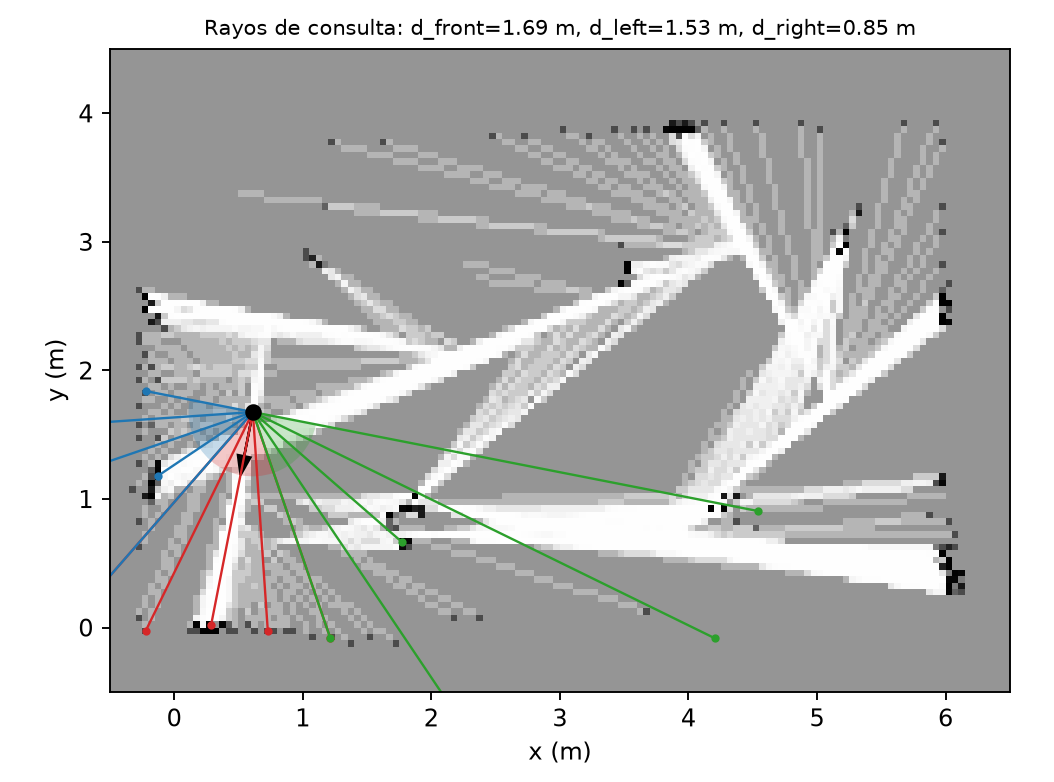
\includegraphics[width=0.75\textwidth]{Capturas_TT2/raycasting_sectores.png}
    \caption{Rayos de consulta por sector sobre el mapa construido en simulación. El
    título indica las distancias resultantes que se entregan al módulo de
    navegación.}
    \label{fig:ray_sectores}
\end{figure}

\begin{center}
\captionof{algorithm}{Distancias libres por sector}
\label{alg:dev_ray_query}
\end{center}
\vspace{-1.8cm}
\rule{\textwidth}{0.4pt}
\vspace{-0.9cm}
\begin{algorithmic}[1]

\Statex \textbf{ENTRADA:} mapa, pose (x, y, $\theta$), alcance\_max = 4 m
\Statex \textbf{SALIDA:} $d_{\text{front}}$, $d_{\text{left}}$, $d_{\text{right}}$

\Statex
\Function{castDistance}{x, y, $\alpha$}
    \For{cada c en bresenham(a\_celda(x, y), a\_celda(x + 4 cos $\alpha$, y + 4 sin $\alpha$))}
        \If{c no es la celda del usuario Y (l(c) $> 1.0$ O peligros(c) $\geq 2$)}
            \State \Return mín(4, distancia(x, y, centro(c)))
        \EndIf
    \EndFor
    \State \Return 4
\EndFunction

\Statex
\For{cada sector (a0, a1) en \{frente: ($-30^\circ$, $30^\circ$), izq: ($30^\circ$, $90^\circ$), der: ($-90^\circ$, $-30^\circ$)\}}
    \State d $\gets$ 4
    \For{k = 0 hasta 4}
        \State d $\gets$ mín(d, castDistance(x, y, $\theta$ + a0 + (a1 $-$ a0) k / 4))
    \EndFor
    \State d\_sector $\gets$ d
\EndFor
\State \Return $d_{\text{front}}$, $d_{\text{left}}$, $d_{\text{right}}$

\end{algorithmic}
\vspace{-0.9cm}
\rule{\textwidth}{0.4pt}

El módulo de navegación utiliza además una versión vectorizada con NumPy del mismo
principio para simular sensores durante el entrenamiento del agente, la cual se
documentará junto con ese módulo.

\subsection{Resultados}

En el banco de simulación, la actualización del mapa con todas las observaciones de un
ciclo (cuatro a seis rayos) tomó en promedio 0.15~ms, y en el procesamiento de video
real, incluyendo el despeje de la huella del usuario, 0.23~ms por ciclo. La
construcción completa del cuadro para navegación, que incluye los quince rayos de
consulta y el mapa local, tomó 0.51~ms. Estos tiempos son dos órdenes de magnitud
menores que el periodo de 100~ms que impone RNF-03, por lo que el Ray Casting no
representa un cuello de botella del sistema.

Para cuantificar la aportación de las reglas añadidas se realizó un experimento de
ablación en el banco de simulación, desactivándolas una por una. Además de la
precisión y la exhaustividad, se contó el número de celdas marcadas como ocupadas que
no tienen ningún obstáculo real a menos de 10~cm (celdas falsas). Los resultados se
muestran en la Tabla~\ref{tab:ray_ablacion}.

\begin{table}[H]
\centering
\caption{Ablación de las reglas del Ray Casting (promedio de seis corridas)}
\label{tab:ray_ablacion}
\renewcommand{\arraystretch}{1.2}
\begin{tabular}{|p{6.0cm}|c|c|c|c|}
\hline
\textbf{Configuración} & \textbf{Precisión} & \textbf{Exhaustividad} &
\textbf{Ocupadas} & \textbf{Falsas} \\
\hline
Vigente (todas las reglas) & 0.60 & 0.31 & 152 & 60 \\
Sin $L_{block}$ & 0.58 & 0.30 & 172 & 73 \\
Rango monocular crudo marca ocupación & 0.60 & 0.32 & 157 & 63 \\
Sin anclar a \emph{landmarks} (rango crudo) & 0.62 & 0.31 & 150 & 57 \\
Sin las tres reglas & 0.57 & 0.35 & 192 & 82 \\
\hline
\end{tabular}
\end{table}

En conjunto, las reglas reducen las celdas falsas de 82 a 60 (alrededor de 27\,\%), y
la mayor parte de esa mejora proviene de $L_{block}$. Quitar las tres reglas sube un
poco la exhaustividad, porque el mapa marca más celdas, pero a costa de más celdas
falsas. Las reglas del rango monocular y del anclaje casi no modifican las métricas
globales del banco, porque la mayoría de las celdas ocupadas corresponden a paredes
registradas por ultrasonido y los objetos son una fracción pequeña del mapa; su
efecto es local, alrededor de cada objeto, donde evitan manchas difusas y marcas
duplicadas. También se observa que cerca del 40\,\% de las celdas ocupadas no
coinciden con un obstáculo real dentro de la tolerancia de 10~cm. La causa principal
no es el Ray Casting sino el error de pose: con un ATE de 0.21~m, una pared registrada
en distintos momentos queda dibujada con un desplazamiento de varias celdas. La Sección~\ref{sec:dev_mapeo}
analiza la calidad del mapa con mayor detalle.

\subsection{Limitaciones}

\begin{itemize}
    \item \textbf{Celdas consolidadas permanentes.} La regla $L_{block}$ impide que un
    rayo de espacio libre atraviese una celda con $l > 2$, lo cual también impide que
    esa celda vuelva a disminuir. En la práctica, una celda que recibió dos o más
    impactos precisos queda marcada como ocupada de forma permanente: se verificó que
    ni cincuenta rayos posteriores que la atraviesan la liberan. Esto significa que
    un obstáculo que desaparece (por ejemplo, una caja que se retira) permanece en el
    mapa, lo cual no cumple por completo con RF-17 en el caso de desaparición de
    obstáculos. Una corrección posible es permitir que los rayos precisos, cuyo
    extremo está claramente más allá de la celda, sí reduzcan su valor.
    \item \textbf{Huecos entre celdas.} Bresenham visita una sola celda por paso, por
    lo que un rayo de consulta diagonal puede pasar entre dos celdas ocupadas que solo
    se tocan por una esquina y reportar libre un frente bloqueado. Esto es frecuente en
    mapas con ecos dispersos. El módulo de navegación lo mitiga lanzando un abanico de
    tres sub-rayos por dirección; una alternativa sería usar el recorrido de
    Amanatides y Woo en la consulta.
    \item \textbf{Mapa bidimensional.} Los rayos se trazan en el plano, por lo que
    obstáculos colgantes (ramas, letreros a la altura de la cabeza) solo se registran
    si los detecta la visión.
    \item Como el rango monocular nunca marca ocupación por sí solo, los obstáculos de
    clases que la visión no reconoce y que no producen eco ultrasónico no aparecen en
    el mapa.
\end{itemize}
